% Copyright (C) 2005-2015 Airbus - EDF - IMACS - Phimeca
% Permission is granted to copy, distribute and/or modify this document
% under the terms of the GNU Free Documentation License, Version 1.2
% or any later version published by the Free Software Foundation;
% with no Invariant Sections, no Front-Cover Texts, and no Back-Cover
% Texts.  A copy of the license is included in the section entitled "GNU
% Free Documentation License".

\renewcommand{\etapemethodo}{C}
\renewcommand{\nomfichier}{docref_C221_MonteCarloStd}
\renewcommand{\titrefiche}{Estimating the mean and variance using the Monte Carlo Method}

\Header

\MathematicalDescription{

  \underline{\textbf{Goal}} \vspace{2mm}

  Let us denote $\underline{Y} = h\left( \vect{X},\vect{d} \right) = \left( Y^1,\ldots,Y^{n_Y} \right)$, where $\vect{X}= \left( X^1,\ldots,X^{n_X} \right)$ is a random vector, and $\vect{d}$ a  deterministic vector. We seek here to evaluate, the characteristics of the central part (central tendency and spread i.e. mean and variance) of the probability distribution of a variable $Y^i$, using the probability distribution of the random vector $\vect{X}$.
  \vspace{2mm}

  \underline{\textbf{Principle}} \vspace{2mm}

  The Monte Carlo method is a numerical integration method using sampling, which can be used, for example, to determine the mean and standard deviation of a random variable $Y^i$ (if these quantities exist, which is not the case for all probability distributions):
  \begin{align*}
    m_{Y^i} = \int u \, f_{Y^i}(u) \, du,\ \sigma_{Y^i} = \sqrt{\int \left( u-m_{Y^i} \right)^2 \, f_{Y^i}(u) \, du}
  \end{align*}
  where $f_{Y^i}$ represents the probability density function of $Y^i$.

  Suppose now that we have the sample $\left\{ y^i_1,\ldots,y^i_N \right\}$ of $N$ values randomly and independently sampled from the probability distribution $f_{Y^i}$; this sample can be obtained by drawing a $N$ sample $\left\{ \vect{x}_1,\ldots,\vect{x}_N \right\}$ of the random vector $\vect{X}$ (the distribution of which is known) and by computing $\vect{y}_j = h \left( \vect{x}_j,\underline{d} \right) \ \forall 1 \leq j \leq N$.
  Then, the Monte-Carlo estimations for the mean and standard deviation are the empirical mean and standard deviations of the sample:
  \begin{align*}
    \widehat{m}_{Y^i} = \frac{1}{N} \sum_{j=1}^N y^i_j,\ \widehat{\sigma}_{Y^i} = \sqrt{\frac{1}{N} \sum_{j=1}^N \left( y^i_j - \widehat{m}_{Y^i} \right)^2}
  \end{align*}
  These are just estimations, but by the law of large numbers their convergence to the real values $m_{Y^i}$ and $\sigma_{Y^i}$ is assured as the sample size $N$ tends to infinity. The Central Limit Theorem enables the difference between the estimated value and the sought value to be controlled by means of a confidence interval (especially if N is sufficiently large, typically $N$ > a few dozens even if there is now way to say for sure if the asymptotic behaviour is reached). For a probability $\alpha$ strictly between 0 and 1 chosen by the user, one can, for example, be sure with a confidence $\alpha$, that the true value of $m_{Y^i}$ is between $\widehat{m}_{i,\inf}$ and $\widehat{m}_{i,\sup}$ calculated analytically from simple formulae. To illustrate, for $\alpha = 0.95$:
  \begin{align*}
    \widehat{m}_{i,\inf} = \widehat{m}_{Y^i} - 1.96 \frac{\displaystyle \widehat{\sigma}_{Y^i}}{\displaystyle \sqrt{N}},\ \widehat{m}_{i,\sup} = \widehat{m}_{Y^i} + 1.96 \frac{\widehat{\sigma}_{Y^i}}{\sqrt{N}},\ \textrm{that is to say}\ \textrm{Pr} \left(  \widehat{m}_{i,\inf} \leq m_{Y^i} \leq \widehat{m}_{i,\sup} \right) = 0.95
  \end{align*}
  The size of the confidence interval, which  represents the uncertainty of this mean estimation, decreases as $N$ increases but more gradually (the rate is proportional to $\sqrt{N}$: multiplying $N$ by 100 reduces the length of the confidence interval  $\left| \widehat{m}_{i,\inf}-\widehat{m}_{i,\sup} \right|$ by a factor 10).

  \begin{center}
    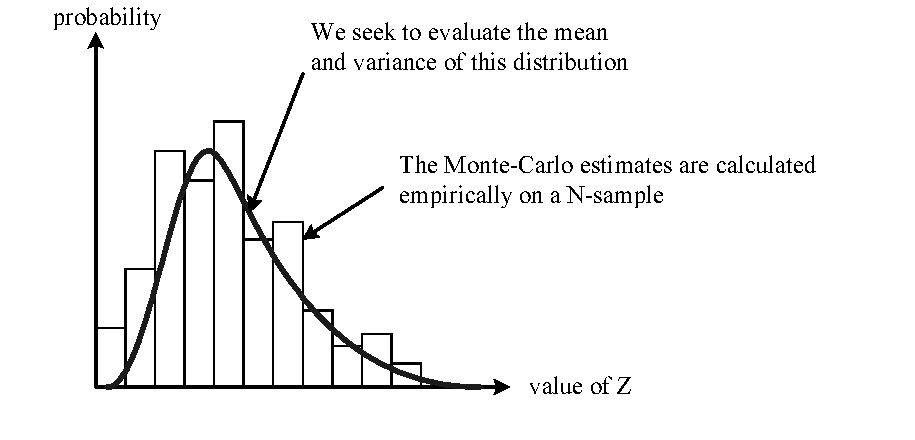
\includegraphics[scale=0.8]{Figures/MC.pdf}
  \end{center}
}
{
  Direct sampling, crude Monte Carlo method, Classical Monte Carlo integration
}

\Methodology{
  In the overall process, the Monte Carlo simulation method for estimating the variance appears in step C "Propagation of Uncertainty" when the study of uncertainty deals with the dispersion of the variable of interest ${Y^i}$ defined in step A "Specifying Criteria and the Case Study". To be more precise, this method requires that the following steps have previously been previously completed:
  \begin{itemize}
  \item step A: specification of input variables $\vect{X}$ and $\vect{d}$ and the output variable of interest $\underline{Y}=h(\vect{X},\vect{d})$,
  \item step B: use of one of the proposed techniques for determining the probability distribution of  the variable $\vect{X}$,
  \end{itemize}

  The method's parameters are the following:
  \begin{itemize}
  \item number $N$ of simulations,
  \item probability $\alpha$ giving the required confidence level for the confidence intervals,
  \end{itemize}

  The method described here returns the following results:
  \begin{itemize}
  \item the Monte-Carlo estimates  $\widehat{m}_{Y^i}$ and $\widehat{\sigma}_{Y^i}$ for the mean and standard deviations of the variable of interest $Y^i$,
  \item the confidence interval $\left[ \widehat{m}_{i,\inf},\widehat{m}_{i,\sup} \right]$ for the mean $m_{Y^i}$.
  \end{itemize}
}
{
  The Monte-Carlo method does not require any assumptions on the form of the function $h$ which relates $\vect{X}$ and $\underline{Y}$, except that the expected value and standard deviation of $Y^i$ should exist (which is not the case, for example, if $Y^i$ follows the Cauchy distribution).

  Actually, the only limitation resides in $N$, the number of simulations, which if not sufficiently high (because of the CPU time required for an estimation of $\underline{Y}=h(\vect{X},\vect{d})$), can result in too greater uncertainty for the estimations of  $\widehat{m}_{Y^i}$ and $\widehat{\sigma}_{Y^i}$. It is fitting then to verify the convergence of the estimators, especially by plotting the graph of the coefficient de variation  $\widehat{\sigma}_{Y^i} / \widehat{m}_{Y^i}$ as a function of $N$: if convergence is not visible, it is necessary to increase $N$ or if needed to choose another propagation method to estimate the central uncertainty of $\underline{Y}$ (see \otref{docref_C211_QuadraticCumul}{Quadratic combination / Perturbation method}).

  The following references provide a bibliographic starting point for interested readers for further study of the method described here:
  \begin{itemize}
  \item Robert C.P., Casella G. (2004). "Monte Carlo Statistical Methods", Springer, ISBN 0-387-21239-6, 2nd ed.
  \item Rubinstein R.Y. (1981). "Simulation and The Monte Carlo methods", John Wiley \& Sons
  \item "Guide to the expression of Uncertainty in Measurements (GUM)", ISO publication
  \end{itemize}
}
